\documentclass[a4paper,12pt]{report}
 
% Différentes options pour la classe :
% - taille de la fonte    : 10pt, 11pt, 12pt
% - recto ou recto-verso    : oneside, twoside
% - stade de développement    : draft, final
 
% Chargement d'extensions
\usepackage[latin1,utf8]{inputenc}    % Pour utiliser les lettres accentuées
\usepackage[francais]{babel}    % Pour la langue française
\usepackage{graphicx}
 
% Informations le titre, le(s) auteur(s), la date
\title{Rapport de projet : Etrange}
\author {Caroline Keramsi, Florian Thorey, Samuel Mokrani}
\date{\today}
 
% Début du document
\begin{document}
 
\maketitle
\tableofcontents    % Table des matières
\listoffigures        % Liste des figures
 
    \chapter*{Introduction}
    \addcontentsline{toc}{chapter}{Introduction}
{Dans le cadre du cours de System On Chips à Télécom Paristech, nous avons du réaliser
un module de traitement vidéo. Plus précisément, ce module doit être capable à partir d'un flux vidéo d'entrée représentée en 256 niveaux de gris, d'établir une transformation géométrique d'ordre 3. Voici les images que nous pouvons obtenir suite à une telle transformation :}
 
\begin{figure}[!h]
	\centering
	\includegraphics[scale = 0.5]{bogart.png}
	\caption{Image non transformée}
\end{figure}

\begin{figure}[!h]
	\centering
	\includegraphics[scale = 0.5]{bogart_tr.png}
	\caption{Image transformée}
\end{figure}

{///////TODO : explication de l'algo backward machin}

	\part{Architecture retenue}
	\section*{Architecture retenue}
	\addcontentsline{toc}{section}{Architecture retenue}
{Pour réaliser ce module de traîtement vidéo, nous avons décidé d'utiliser l'architecture suivante :
 
\begin{figure}[!h]
	\centering
	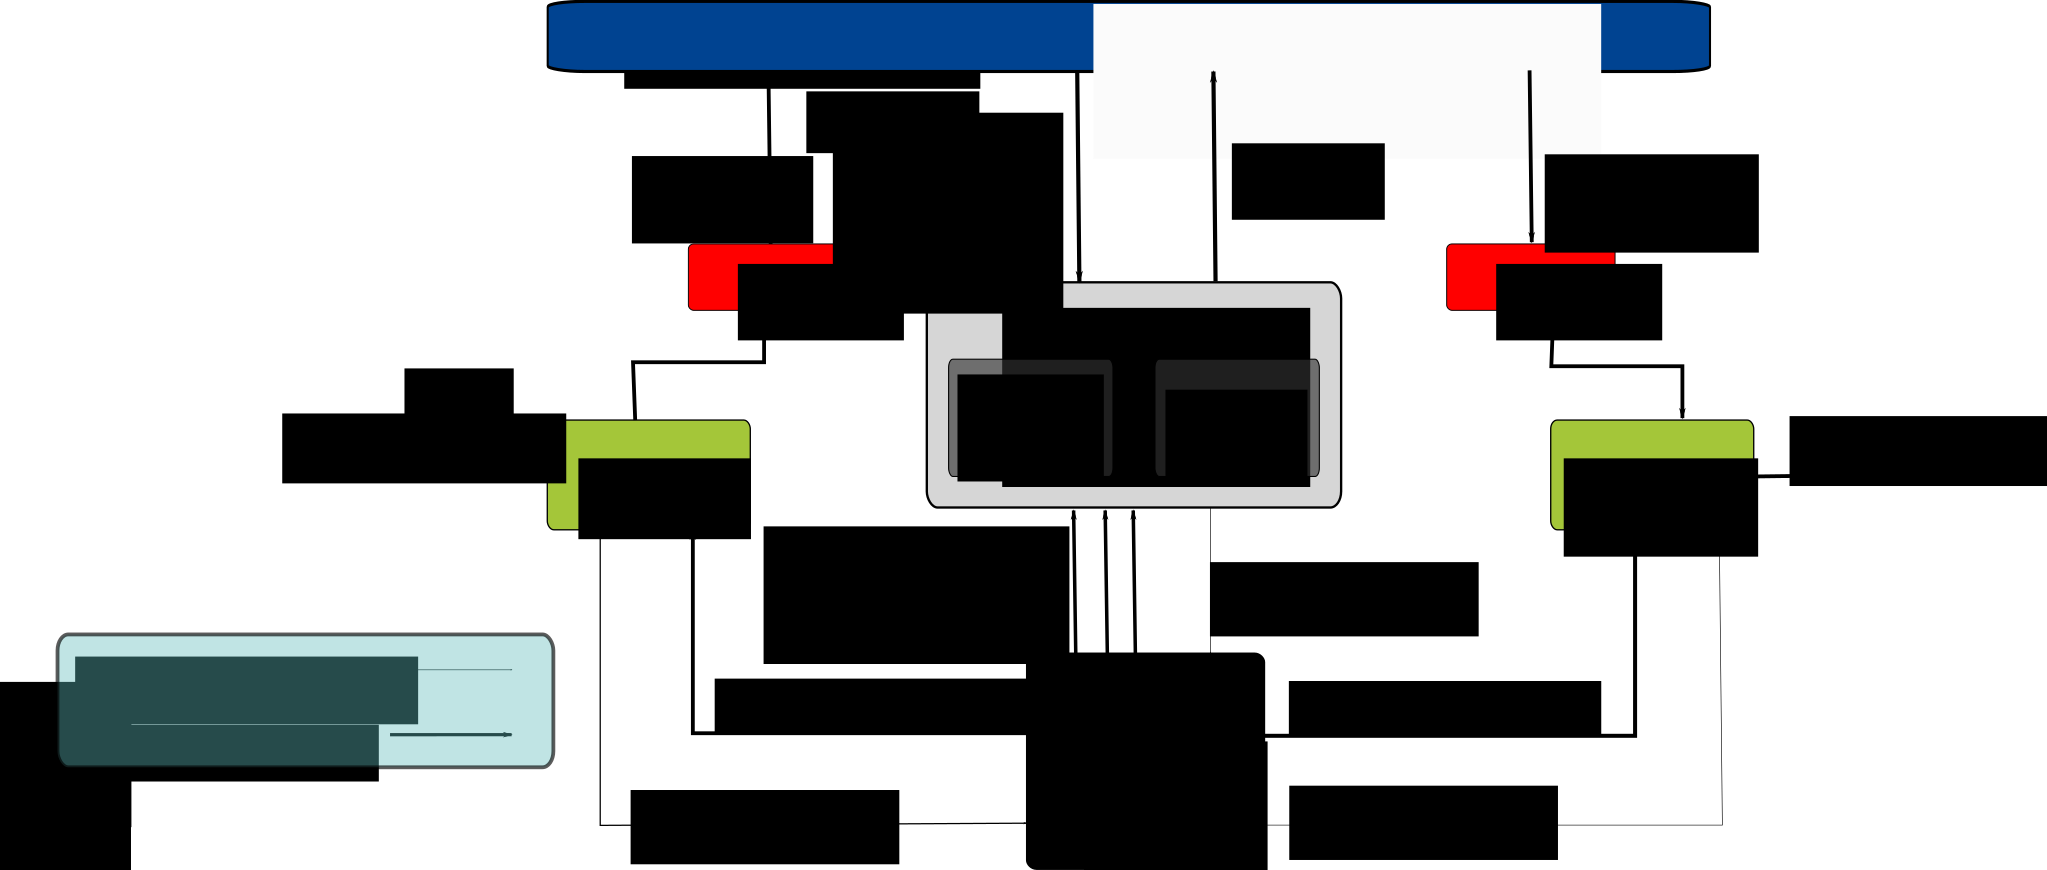
\includegraphics[scale = 0.1]{hardware-arch.png}
	\caption{Architecture}
\end{figure}

Le module VidéoIn se charge de mettre le flux entrant en RAM. VidéoCalc se charge d'aller lire en RAM une image à traîter et à mettre à un autre endroit de la RAM l'image traîtée. Enfin, le module VidéoOut se charge d'aller lire l'image traîtée et de générer un nouveau flux vidéo. Tous ces modules seront pilotés par le processeur (LM32) par le biais d'interruptions. Il enverra aux différents modules les bonnes adresses pour aller lire et écrire en RAM.


Cette architecture a l'avantage d'être modulaire. Par exemple, on peut ne pas utiliser le module de transformation juste en changeant le programme tournant sur le processeur.
}






    \part{VidéoIn / VidéoOut}

    \section*{VidéoIn}
    \addcontentsline{toc}{section}{VidéoIn}

\begin{figure}[!h]
	\centering
	\includegraphics[scale = 0.5]{video_in.png}
	\caption{Architecture de VidéoIn}
\end{figure}

Le rôle du module VidéoIn est de lire le flux vidéo entrant puis de stocker les images correspondantes en RAM à l'adresse spécifiée par le processeur.
VidéoIn est constitué de deux sous-modules qui correspondent à ces deux fonctions et qui permettent de les exécuter en parallèle. 


\subsection*{Module read}
Le premier, read, prend en entrée le flux vidéo constitué du pixel à lire sur 8 bits et des signaux de synchronisation line\_valid et frame\_valid.
Lorsqu'il a détecté un pixel valide, il le place dans une fifo pour le mettre à disposition du module store.
La synchronisation entre le module read et le module store est un point délicat. 
En effet la fifo contient uniquement des pixels et ne transportent aucune information concernant leur position dans l'image. 

\paragraph*{SystemC}
En systemC store est implémenté avec un sc\_thread. Il peut ainsi disposer de ses propres compteurs qui lui permettent de se souvenir de la position
du pixel courant dans le flux vidéo.

\paragraph*{SystemVerilog}

\subsection*{Module store}
Pour commencer, le module store attend que le processeur lui ait fourni une adresse. Pour ce faire il surveille le registre de contrôle du module wb\_slave
qui lui est dédié. Quand celui-ci passe à 1, le module échantillone le contenu du registre d'adresse réservé à VidéoIn. 
Store rentre ensuite dans la phase de stockage d'une image.
Il attend que NB\_PACK pixels soient présents dans la fifo. Dès que c'est le cas, il les lit et les regroupe par paquets de 4, soit 32 bits,
pour les stocker dans la RAM par une écriture wishbone bloc. 
Lorsqu'il a fini d'écrire une image, le module envoie une interruption au CPU et se met en attente d'une nouvelle adresse.
//TODO à vérifier, peut-être à implémenter
//TODO Mettre les mêmes noms de constantes et les mêmes valeurs entre systemC et systemVerilog//


{}

\newpage
 
    \section*{VidéoOut}
    \addcontentsline{toc}{section}{VidéoOut}

{}
     








    \part{VidéoCalc} 
    \section*{VidéoCalc}
    \addcontentsline{toc}{section}{VidéoCalc}

{}










    \part{Soft (LM32)} 

    \section*{Soft (LM32)}
    \addcontentsline{toc}{section}{Soft (LM32)}

{Le processeur a la charge d'indiquer aux différents modules les adresses à aller lire et écrire les images. Plus précisément :

\begin{itemize}
	\item VidéoIn : envoie de l'adresse où l'image entrante sera stockée
	\item VidéoCalc : \begin{itemize}
								\item envoie de l'adresse où sera lue l'image à traitée
								\item envoie de l'adresse où sera stockée l'image traîtée
								\item envoie de l'adresse du début des coefficients pour le calcul incrémental
							\end{itemize}
	\item VidéoOut : envoie de l'adresse où sera lue l'image traîtée
\end{itemize}

Toutes ces adresses sont envoyées suites à des interruptions.
}



 
    \chapter*{Conclusion}
    \addcontentsline{toc}{chapter}{Conclusion}
{}


% Fin du document
\end{document}
